\documentclass[10pt]{article}
\usepackage{siunitx}
\usepackage{amsmath}
\usepackage{amssymb}
\usepackage{amsfonts}
\usepackage[colorlinks,allcolors=black]{hyperref}
\usepackage{booktabs}
\usepackage{graphicx}
\usepackage{subfigure}
\usepackage{float}
\usepackage{url}
\usepackage{multirow}
\usepackage{amsthm}
\usepackage{threeparttable}
\usepackage[linesnumbered,boxed,ruled,commentsnumbered,noend]{algorithm2e}
\usepackage{color}
\usepackage{cancel}
\usepackage{ulem}
\normalem
% GENERAL
\usepackage{xcolor}
\newcommand{\todo}[1]{\textcolor{red}{TODO: #1}}
\newcommand{\improve}[1]{\textcolor{cyan}{IMPROVE:#1}}
\newcommand{\note}[1]{\textcolor{blue}{NOTE: #1}}
\newcommand{\respond}[1]{\textcolor{purple}{RESPOND: #1}}
\newcommand{\question}[1]{\textcolor{orange}{Q: #1}}
\newcommand{\changed}[1]{\textcolor{red}{#1}}

\usepackage{indentfirst}



%%%%%%%%%%%%%%%%%%%%%%%%%%%%%%%%%%%%%%%%
\begin{document}
\title{Authors' Response for Submission ``Time Minimization and Online Synchronization for Multi-agent Systems
	under Collaborative Temporal Logic Tasks''}
\author{Zesen Liu, Meng Guo, and Zhongkui Li}
\date{}
\maketitle



\section*{To Associate Editor}


\textbf{C:}
\emph{The paper proposes a method for collaborative multi-agent planning
under timed temporal tasks. Two reviews were collected a summary of
which is as follows. Reviewer 5 provides a long list of technical
comments, some of which question the correctness of some of the
results, eg the proofs of Lemmas 1 and 2. Reviewer 6 is concerned about
the presentation and writing and provides a list of relevant comments.
Some technical comments are found therein as well. Based on the reviews
and my own reading, a thorough revision is in order. This should take
both the technical and presentation related queries of the reviewers
into account.
}

\textbf{A:}
The authors are grateful to the Associate Editor for handling our submission and the insightful suggestions.
We have mainly made the following modifications accordingly:
\begin{itemize}
\item Suggestions given by reviewers are fully addressed.
  For instance, the communication protocol between leaders and followers
  as suggested by Reviewer 5
  is added into the online adaptation part;
  more active tones are adopted in Introduction as suggested by Reviewer~6;
 discussions for future work are extended as suggested by both Reviewers~5,6;
  and the description of Lemma~2 and its proof are improved as suggested by Reviewer~5.

\item As suggested by both reviewers,
  more details and explanations are added in the proposed task assignment algorithm,
  where the heuristics during the node expansion and the design of lower
  and upper bounds are described with more care.
  Further examples are added to clarify the technical questions
  raised by both reviewers regarding the design of these heuristics.

\item Numerous typos are corrected as pointed out by the reviewers, e.g., in the abstract and preliminaries.
\end{itemize}
All these changes have been highlighted in blue in the revised paper.
Detailed responses to each reviewer can be found in the sequel.
$\hfill\blacksquare$



%===========================================================


\newpage
\section*{To Reviewer 5}

\textbf{C:}
\emph{This manuscript proposes a framework for online motion planning for
	multi-agent systems under collaborative temporal logic tasks. The
	proposed framework consists of three main parts as the main
	contributions of this manuscript. The three parts are as follows. 1.
	The authors propose a new method to convert a given sc-LTL
	specification to a partially ordered set namely "poset" that captures
	the temporal constraints of the given sc-LTL formula and then they
	propose an anytime algorithm to synthesize the motion and action
	sequence for the given specification. 2. They propose a method based on
	BnB approach for assigning the synthesized actions to the agents. 3.
	Then, they propose an online adaptation method in case of changes in
	the work environment or the failure of some of the agents. }

\emph{	The authors provided Lemmas and Theorem to prove the correctness and
	completeness of the proposed methods and algorithms. In addition,
	different aspects of the proposed methods and algorithms are compared
	to the existing works in the literature to emphasize the advantages and
	novelties of the proposed framework. Overall, this manuscript provides
	a new and comprehensive framework for motion planning for multi-agent
	systems under collaborative temporal logic tasks with extensive case
	studies.  However, there are some ambiguities to be clarified in the
	manuscript. Below, a list of detailed comments is provided.}

\textbf{A:}
The authors thank the reviewer for the constructive comments and insightful suggestions.
They helped us greatly improve the submission and further strengthen its contributions.
Below we summarize our replies to these comments, accompanied by the list of changes in the revision.
All these changes have been highlighted in blue in the revised paper.
$\hfill\blacksquare$
%我们根据你的意见修改了什么的地方+内容
%针对这个review 改了什么地方

\hspace*{\fill} \

%===========================================================

\textbf{C:}
\emph{In the proof of Lemma 1, it is assumed that the associated accepting
	run of $\mathcal{B}$ is $\rho=...q_1q_3...$ . Is this assumption compatible
	with the definition of the accepting run? The proof needs to be more
	elaborated. For example, why is it assumed that $q_2$ is not in the
	accepting run of $\mathcal{B}$?}

\textbf{A:} Thank you for your suggestion.
By definition, the associated run of an accepting word is the accepting run of $\mathcal{B}$.
The subscript ``$2$'' of $q_2$ is used to distinguish different states, which does not indicate the relative order of states $q_1,q_2,q_3$.
In other words,
we can also assume that the accepting run of $\mathcal{B}$ is given by~$\rho=\cdots q_1q_2\cdots$ and the accepting run of $\mathcal{B}^-$
is given by~$\rho=\cdots q_1q_3q_2\cdots$.

The proof of Lemma 1 has been improved as follows:
\begin{itemize}
\item In line 2 of the proof of Lemma 1, right column, Page 5, we change the subscripts of $\rho$ such that given an accepting word $w=\cdots\{\sigma_n\}\cdots$, its accepting
 run in $\mathcal{B}$ is given by {$\rho=\cdots q_{i}q_{j}\cdots$},
 with {$q_{j}=\delta(q_i,\sigma_n)$}.

\item In lines 3-6 of the proof of Lemma 1, right column, Page 5,  we add Case 1 that if no edges in $\rho$ are \emph{Decomposable Transitions}, all edges in $\rho$
can be found in $\mathcal{B}^-$. In other words, $\rho$ is accepting in $\mathcal{B}^-$.


\item In lines 12-16 of the proof of Lemma 1, right column, Page 5, we add discussions about the relation between Case 1 and Case 2. Specifically,
if the transitions from $q_k$ to $q_j$ and from $q_i$ to $q_k$
are not removed in $\mathcal{B}^-$, this satisfies Case 1 and $w'$ is the associated accepting path in $\mathcal{B}^-$.
 If any transition is removed as a \emph{Decomposable Transition}, it satisfies Case 2 and an additional time step is added.

\item In lines 17-19 of the proof of Lemma 1, right column, Page 5, we add the explanation why Case 2 eventually becomes Case 1.
  Namely, according to {Definition~2}, it eventually happens in Case 2 that the new created run $\rho'$ has no \emph{Decomposable Transition}, thus satisfying the condition of Case 1.
\end{itemize}
$\hfill\blacksquare$


\hspace*{\fill} \



%===========================================================

\textbf{C:}
\emph{In the paragraph below Def. 3, the meaning of the notation of
	$\sigma_{\ell}^{-}$ is not clear at all. What does s mean in
	$\forall{s}\in{\sigma_{\ell}}$? What does superscript s mean?}

\textbf{A:} Thanks for your insightful comment. It is our mistake that the same symbol ``$s$''
is used to denote both the superscript and labels.
The superscript $s$ in $\sigma^s$ is the initial of ``\emph{self loop}''
to indicate that $\sigma^s$ contains the self-loop constraints.
On the other hand, the $s$ in $\forall{s}\in{\sigma_{\ell}}$
is a label from the set of labels~$\sigma_{\ell}$.
To avoid confusion,
the latter has been changed to~$z$ instead, i.e., $\forall{z}\in{\sigma_{\ell}}$.
We have also modified the definition of $\sigma^s$ to
give a more clear description that $\sigma^s$ is the set of labels
that will invalidate the self-loop transition.
Specifically, Definition~3 has been modified as follows:
\begin{itemize}
\item In line 7 of Definition~3, left column, Page 6,
  it is clarified that $q_{\ell} \notin \delta(q_{\ell-1},\,\sigma^-_\ell)$
  holds for case (ii), where~{$\sigma^-_\ell =  \sigma_\ell \backslash \{z\}$, $\forall z\in \sigma_\ell$},"

\item In line 9 of Definition 3, left column, Page 6,
  two cases are further extended, namely,
(i) $q_{\ell-1} \notin \delta(q_{\ell-1},\,\sigma)$, for all $\sigma\in\Sigma, \sigma\cap\sigma^{s}_\ell\neq\emptyset$;
and (ii) $q_{\ell-1} \in \delta(q_{\ell-1},\,\sigma)$, for all  $\sigma\in\Sigma, \sigma\cap\sigma^{s}_\ell=\emptyset$.
\end{itemize}

%==============================
\begin{figure}[ht]
	\centering
	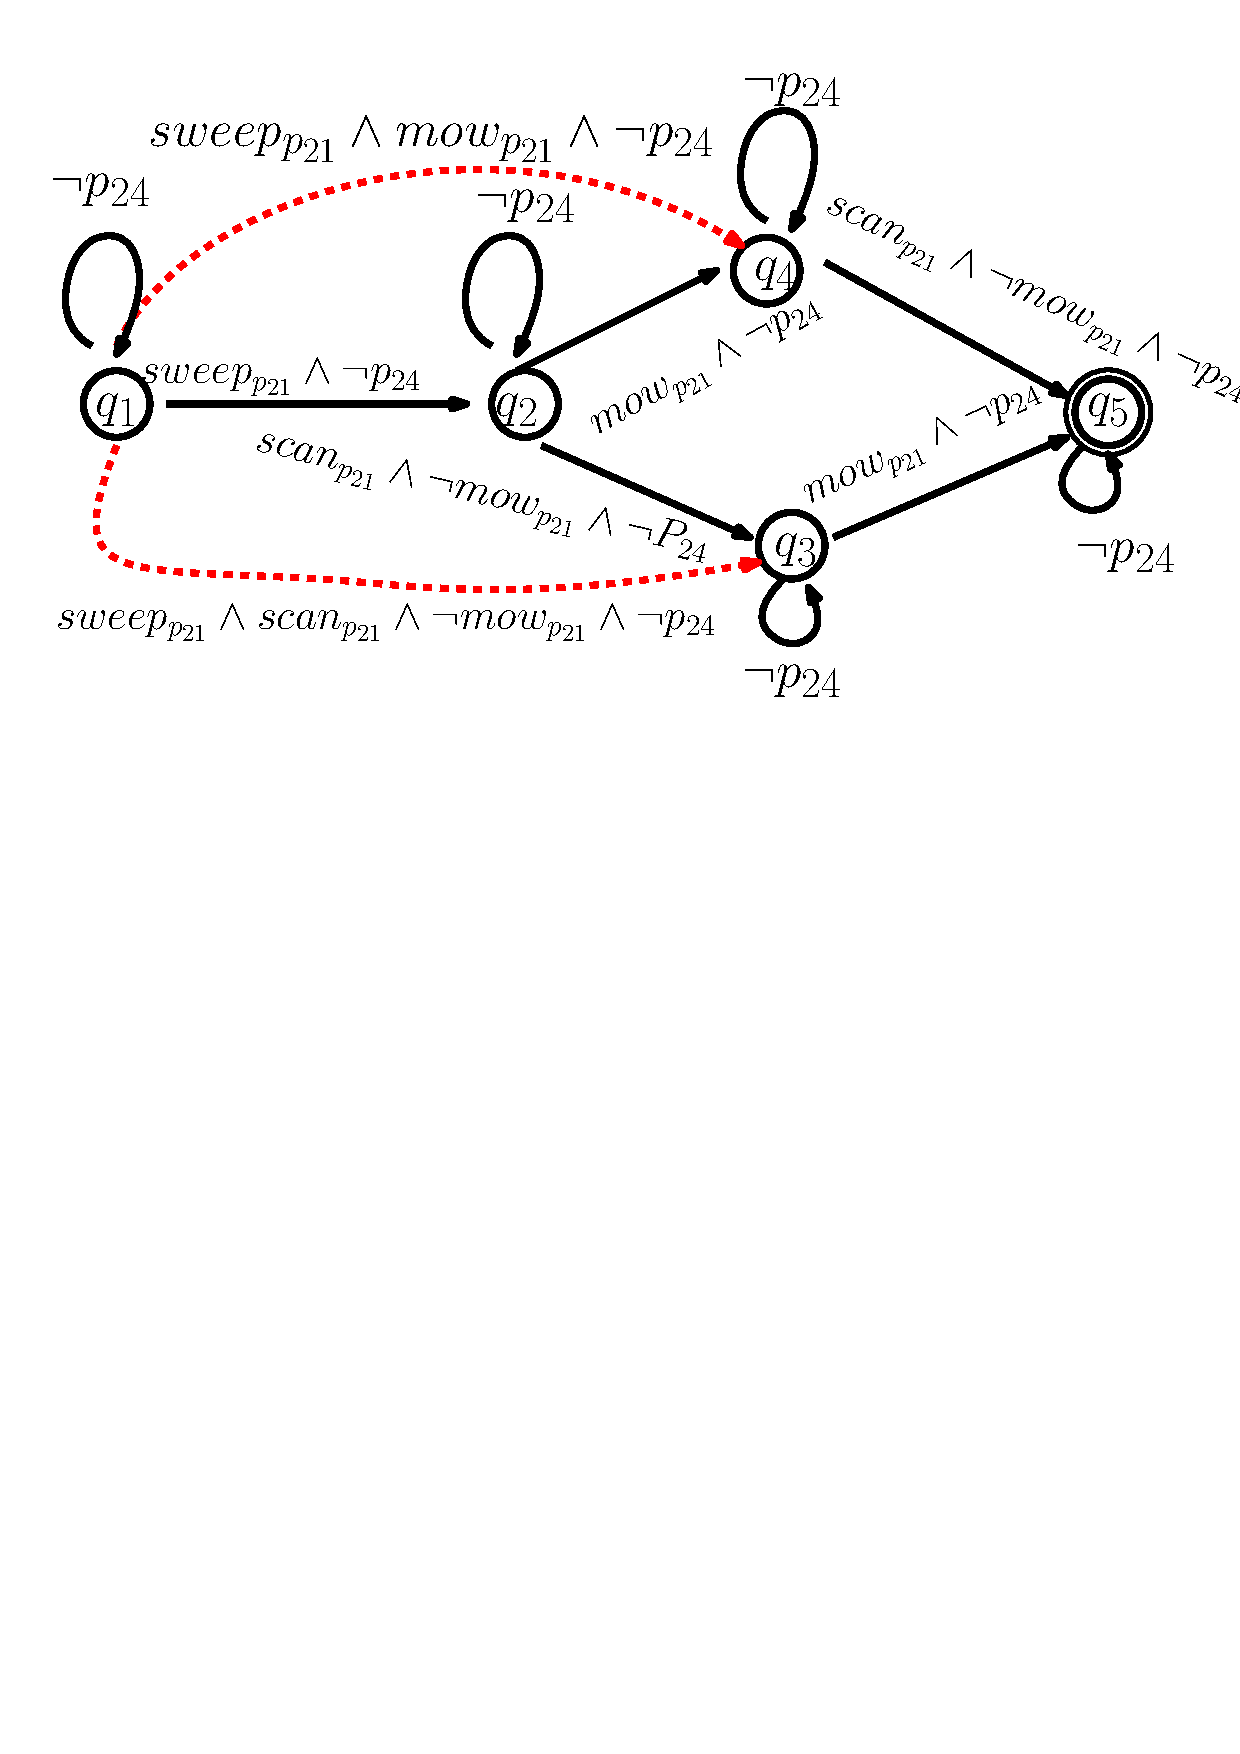
\includegraphics[scale=0.35]{figs/example_decomposable.pdf}
	\caption{Example of a pruned B\"{u}chi automata.}
	\label{fig:example_decomposable}
\end{figure}
%==============================

For instance, an example of a pruned NBA $\mathcal{B}_{\varphi}^-$ is shown in the above Figure~\ref{fig:example_decomposable}.
We can find an accepting run with $\rho=q_1q_2q_4q_5$.
One \emph{possible} decomposition of the subtasks is given by $\Omega_\varphi=\{(1,\{\texttt{sweep}_{\texttt{p}_{21}}\},\{ \texttt{p}_{24}\}),
(2,\{\texttt{mow}_{\texttt{p}_{21}}\}, \{\texttt{p}_{24}\}),\\
(3, \{\texttt{scan}_{\texttt{p}_{21}}\}, \{ \texttt{p}_{24}\})\}$.
Regarding subtask $\omega_1$, $\sigma_1=\{\texttt{sweep}_{\texttt{p}_{21}}\}$ and
the associated $\sigma^-_1=\{\}$ can be created by removing the label $\texttt{sweep}_{\texttt{p}_{21}}\in \sigma_1$.
It holds that $q_2\notin \delta(q_1,\{\})$, $q_2\in\delta(q_1,\{\texttt{sweep}_{\texttt{p}_{21}}\})$.
Furthermore, $\sigma^s_1=\{\texttt{p}_{24}\}$ means that the set of labels
$\sigma=\{\texttt{sweep}_{\texttt{p}_{21}}, \texttt{p}_{24}\}$ cannot satisfy
the condition of a self-loop transition $q_1\notin \delta(q_1, \{\texttt{sweep}_{\texttt{p}_{21}}, \texttt{p}_{24}\})$ because $\sigma^s_1\cap\sigma\neq\emptyset$, while
$\sigma=\{\texttt{sweep}_{\texttt{p}_{21}}\}$ satisfies the condition of a self-loop
transition $q_1\in \delta(q_1,\{\texttt{sweep}_{\texttt{p}_{21}}\})$ because
$\sigma^s_1\cap\sigma=\emptyset$.

Example 3 on Page 6 has been modified accordingly.
{For subtask $\omega_1$, $\ell=1$, $\sigma_1=\{\texttt{sweep}_{\texttt{p}_{21}}\}$ and $\sigma^s_1=\{\texttt{p}_{24}\}$,
$\sigma^-_1$ can be $\{\}$, which satisfies that $q_2\notin
	\delta(q_1,\sigma^-_1)$, $q_2\in\delta(q_1,\sigma_1)$.
Furthermore, for $\sigma=\{\texttt{sweep}_{\texttt{p}_{21}}, \texttt{p}_{24}\}$ and $\sigma\cap\sigma^s_1\neq\emptyset$, there exists $q_1\notin \delta(q_1, \{\texttt{sweep}_{\texttt{p}_{21}}, \texttt{p}_{24}\})$.
For $\sigma=\{\texttt{sweep}_{\texttt{p}_{21}}\}$ and $\sigma\cap\sigma^s_1=\emptyset$, there exists $q_1\in \delta(q_1,\{\texttt{sweep}_{\texttt{p}_{21}}\})$.}
$\hfill\blacksquare$

\hspace*{\fill} \



%===========================================================

\textbf{C:}
\emph{In Example 3, why are the indices of all three tasks 1? Aren't these
	different subtasks?
}

\textbf{A:}  Thanks for this detailed comment.
We have fixed the typo by using different indices for different subtasks,
i.e., $\{(1,\{\texttt{sweep}_{\texttt{p}_{21}}\},\{\texttt{p}_{24}\}),
(2,\{\texttt{mow}_{\texttt{p}_{21}}\}, \{\texttt{p}_{24}\})$,
$(3, \{\texttt{scan}_{\texttt{p}_{21}}\}, \{ \texttt{p}_{24}\})\}$.
$\hfill\blacksquare$


\hspace*{\fill} \

%===========================================================

\textbf{C:}
\emph{Why are the notations $\omega$ and $\sigma$ used for referring to
	subtasks interchangeably?}

\textbf{A:} Thanks for pointing out the ambiguity.
We have unified the terminologies that $\omega_\ell\in \Omega_\varphi$ are referred
as ``subtasks" while $\sigma_\ell\in \Sigma$ are ``labels".
More specifically, the modifications are as follows:
\begin{itemize}
\item In line 6 of Definition 3, left column, Page 6, it is emphasized that $\ell$ is the index of subtask {$\omega_\ell$}, and {labels} $\sigma_\ell\subseteq\Sigma$ satisfies two conditions.

\item In the last paragraph, left column, Page 6, it is added that
  a {subtask $\omega_\ell=(\ell,\,\sigma_\ell,\sigma^s_\ell)$} consists of
  its index, a set of action propositions labels and
  a set of self-loop requirement labels.

\item In the last paragraph, left column, Page 6, it is clarified that the two conditions of label $\sigma_\ell$ in the above definition are required for
  each label $\sigma_\ell$ of subtask $\omega_\ell$.
\end{itemize}

$\hfill\blacksquare$




\hspace*{\fill} \

%===========================================================

\textbf{C:}
\emph{In Def. 4,  what are the limitations on the number of tasks that can
	be executed at the same time?
}

\textbf{A:}
Thanks for this comment.
The number of tasks that can be executed at the same time is upper bounded by $|\Omega_\varphi|$.
For instance, consider the formula $\varphi=\Diamond (\alpha_1 \land \neg (\alpha_2 \land \alpha_3) )\land \Diamond \alpha_2 \land \Diamond \alpha_3$.
The associated R-poset is given by~$P=(\Omega_\varphi, \preceq_\varphi, \neq_\varphi)$,
 with $\Omega_\varphi=\{\omega_1=(1,\{\alpha_1\},\{\}),
 \omega_2=(2,\{\alpha_2\},\{\}),
 \omega_3=(3,\{\alpha_3\},\{\})
 \}$, $\preceq_\varphi=\{\}$, $\neq_\varphi=\{\{\omega_1,\omega_2,\omega_3\}\}$.
We can find that $\{\omega_1, \omega_2\}$  and $\{\omega_2, \omega_3\}$ can be executed at the same time.
However, $\{\omega_1,\omega_2,\omega_3\}$ cannot be executed at the same time due to the constraints imposed by $\neg (\alpha_2\land\alpha_3)$.
Thus, $\{\omega_1,\omega_2,\omega_3\}$ is added to $\neq_\varphi$ and
the number of tasks that can be executed at the same time is upper bounded by~$2$. On the other hand,
consider the formula $\varphi=\Diamond \alpha_1 \land \Diamond \alpha_2 \land \Diamond \alpha_3$, we can get the same set of subtasks $\Omega_{\varphi}$
and the relation that $\neq_\varphi=\emptyset$, which means that these three subtasks can be executed at
the same time. Generally speaking, the number of tasks that can be executed
at the same time is restricted by the elements of the $\neq_\varphi$ relation,
which is upper bounded by~$|\Omega_{\varphi}|$.
$\hfill\blacksquare$

\hspace*{\fill} \

%===========================================================

\textbf{C:}
\emph{In Line 8 of Algorithm 1, $Que$ is not clearly defined.
}

\textbf{A:} Thanks for this comment.
$Que=[w]$ is a queue to store the accepting words $w$
which can be found in Lines 9-19 of Algorithm 1.
It is also used in the termination condition in Line 9,
which indicates that all words in $L(P)$ have been found.
To avoid ambiguities, Line 8 of Algorithm 1 has been modified to
``Set $L(P)=\{w\}$, $Que=[w]$, $I_1=I_2=\emptyset$''.
Moreover, we have added the following clarifications on Page 7, right column:
``the queue $Que$ is used to store the accepting words $w$
and the iteration ends when $|Que|=0$ in Line~9,
which indicates that all words in $L(P)$ have been found.''
$\hfill\blacksquare$


\hspace*{\fill} \

%===========================================================

\textbf{C:}
\emph{In the proof of Lemma 2, how can you guarantee that there always
	exists a sequence of switching operations in Line 13 of Algorithm 1?
	This claim has been used in the proof of Lemma 3 as well. More
	elaboration is needed on this claim.
}

\textbf{A:} Thank you for this valuable comment.
We can give a constructive approach similar to the bubble sorting algorithm,
in order to find a sequence of switching operations.
Assume that there exists a word $w\in L_{\varphi}$ that satisfies $P$ but $w\not\in L(P)$, i.e., $w$ satisfies the partial ordering constraints in~$P$ but does not belong to $L(P)$. Regarding the ordering relation~$\preceq_{\varphi}$,
due to the iteration process of~$Que$ in Lines~9-18 of Algorithm 1,
any accepting word~$w$ that can be generated by a sequence of switching operation will be added
to~$L(P)$. Assuming that $w=\sigma_j\sigma_k\cdots$
where $w[1]$ is associated with the subtask~$\omega_j$,
we can infer that $(\omega_i,\omega_j)\notin \preceq_\varphi$ holds if $i<j$
and $w$ cannot satisfy the less equal constraints.
Similar to the bubble sorting algorithm,
$w_o[j]$ is switched sequentially with all the preceding terms $w_o[j-1],\cdots,w_o[0]$.
The resulting word $w'$ after each switch is accepting, because
if $w'$ is not accepting, then the switched subtask pair
$(\omega_i,\omega_j)$ is kept in $\preceq_\varphi$ for all $i<j$ as in Line 19.
Afterwards, the resulting word is given by~$w_1=\sigma_j\sigma_1\sigma_2\cdots$.
This operation can be applied to relocate $\sigma_k$ in $w_1$ to the second
place as $w_2=\sigma_j\sigma_k\sigma_1\sigma_2\cdots$, and so on until~$w_n=w$ holds.
Thus, every word generated in the process is accepting,
and the resulting~$w$ is added to $L(P)$.
The above descriptions about how to derive the switching sequence
have been added into the proof of Lemma~2.
$\hfill\blacksquare$


\hspace*{\fill} \

%===========================================================

\textbf{C:}
\emph{In Lemma 3, the notation ``$\subset\subset$'' is not defined.
}

\textbf{A:} Thanks for pointing out this typo.
We have fixed it in the revision.
$\hfill\blacksquare$

\hspace*{\fill} \

%===========================================================


\textbf{C:}
\emph{On Page 9, left column, it is written that "To avoid producing
	infeasible.....". What does it mean that only the next task satisfies
	the partial ordering and how does it help with avoiding producing
	infeasible nodes?
}

\textbf{A:} Thanks for this insightful comment.
The purpose of obeying the partial ordering during task assignment
is to avoid assigning subtasks to one agent in the order that clearly
violates the partial ordering constraints. A node is infeasible,
if the current assignment of one agent $n$ as $\tau_n=\cdots\omega_j\cdots\omega_i\cdots$ violates the partial relation $(\omega_i,\omega_j)\in\preceq_\varphi$.
In this case, any subsequent child node would be infeasible.
Thus, removing the infeasible nodes directly from the search space can
improve search efficiency.

For instance,
consider a R-poset with $P=\{\Omega=\{\omega_1,\omega_2,\omega_3,\omega_4\},
\preceq=\{(1,2),\\(1,3),(3,4)\}, \neq=\{\{1,3\}\}\}$ and a system of three agents.
Via Algorithm 3, the first node is given by~$\nu_0=((),(),())$.
To begin with, $\omega_1$ is available to be assigned as~$Pre(\omega_1)=\{\}$.
Then, several child nodes can be expanded as
$\nu_1=((\omega_1),(),())$, $\nu_2=((),(\omega_1),())$, $\nu_3=((),(),(\omega_1))$.
For node $\nu_2$, subtasks $\omega_2,\omega_3$
can be assigned, since their parent subtasks $Pre(\omega_2)=Pre(\omega_3)=\{\omega_1\}$ have been assigned.
In contrast, if the tasks are assigned regardless of their partial ordering, e.g.,
$\nu_0$ is expanded to $\nu_4=((\omega_4),(),())$ by assigning subtask~$\omega_4$, then
$\nu_4$ cannot be expanded to $\nu_5=((\omega_4, \omega_3),(),())$ by assigning~$\omega_3$,
since it would violate the partial ordering constraint~$(\omega_3,\omega_4)\in\preceq$.

The above explanations ave been added into the manuscript.
Please refer to the colored sentences in the last paragraph, right column, Page 9.
$\hfill\blacksquare$

\hspace*{\fill} \

%===========================================================
\textbf{C:}
\emph{In the paragraph below Eq. 10, it is written that "Once this
  subtask $\omega$ is chosen, the succeeding or child node...".
  How are the
	requirements for being in a certain region for executing a certain task
	taken into consideration when assigning actions to agents with "capable
	function"? Also, the phrase "capable function" seems vague.}


\textbf{A:} Thanks for this insightful comment.
Regarding the first question,
the requirements for being in a certain region to execute a
collaborative task is considered in the ``bounding'' process,
rather than in the current iteration
of \emph{node expansion}.
In other words, the child nodes are expanded by assigning subtask $\omega$ to
each agent that is capable of performing this subtask,
since an agent can always transit to the target region with different time cost.
This guarantees that all child nodes can be visited.
Then, in the step of \emph{lower and upper bound},
the lower bounds of these newly-created child nodes are checked.
Regarding one child node, assume that there is an agent $n$ at its initial region $\texttt{p}_{i}$
which is assigned with task $\tau_n=\cdots\omega_j\omega_k\cdots$ with
$\omega_j=(j, \{\texttt{wash}_{\texttt{p}_{j}}\}, \{\}), \omega_k=(k, \{\texttt{mow}_{\texttt{p}_k}\},\{\})$.
The time cost of agent $n$ to transit to the target region is obtained from the transition graph, i.e., $\mathcal{G}_n=({\mathcal{W}},\,\rightarrow_n,\,d_n)$, as $t_{tran}=d_n(\rightarrow_n(\texttt{p}_{i},\texttt{p}_{j}))$, where $\rightarrow_n\subseteq {\mathcal{W}}\times {\mathcal{W}}$
is the allowed transition for agent~$n$,
and $d_n:\rightarrow_n \rightarrow \mathbb{R}_{+}$ maps each transition to its time duration.
These clarifications have been added on Page 4, left column.

Consequently, the transition time is derived via an optimization:
$$t_j\geq d_n(\rightarrow_n(p_i,p_j)),$$
and $$t_k\geq d(\texttt{wash}_{\texttt{p}_{j}})+t_j+d_n(\rightarrow_n(p_j,p_k)) ,$$
where $t_j,t_k$ are the starting time instants of $\omega_j,\omega_k$, respectively,
$d(\texttt{wash}_{\texttt{p}_{j}})$ is the duration of executing behavior $\texttt{wash}_{\texttt{p}_{j}}$,
and $d_n(\rightarrow_n(p_i,p_j)), d_n(\rightarrow_n(p_j,p_k))$ are the time cost of two transitions.
It is worth mentioning that the transition graph~$\mathcal{G}_n$ is already
constructed offline before the task assignment.
The detailed changes are as follows:
\begin{itemize}
\item In the last paragraph, left column, Page 10, it is clarified that
  the makespan $T_\nu$ is calculated given
  the temporal constraints within the R-poset, dynamic constraints of agents, and the conditions of collaborative subtasks.

\item In particular, the condition $(\omega_i,\omega_j)\in\preceq_\varphi$ requires that subtask~$\omega_j$
  should start being executed only after $\omega_i$ is started;
  $\{\omega_i,\omega_j\}\in\neq_\varphi$ requires that the execution time of $\omega_i, \omega_j$ must not overlap;
  the dynamic constraints require that agent $n$ needs to follow the transition
  cost between different regions in graph~$\mathcal{G}_n$;
  and the collaborative constraints require that all actions of
  one cooperative behavior should be executed simultaneously.
\end{itemize}

Regarding the second question, as mentioned in Equation (1) on Page 4,
a collaborative behavior requires a set of collaborative actions:
$$C_k\triangleq \{a_1,\,a_2,\cdots,a_{\ell_k}\},$$ and each agent
is capable of performing a set of actions $\mathcal{A}_n$.
Thus, an agent~$n$ can participate in the collaborative behavior
if $\mathcal{A}_n\cap C_k\neq \emptyset$.
Moreover, to build a new child node by assigning a subtask $\omega_i$
that is associated with the collaborative behavior $C_k$,
each collaborative action must be assigned to a different agent.
For instance, the subtask $\omega_1=(1,\{\texttt{repair}_{\texttt{p}_{24}}\},\{\})$
requires two collaborative actions $\texttt{repair}_s$ and $\texttt{repair}_l$
to be executed at region $\texttt{p}_{24}$.
Since agents of type $V_l$ are capable of action~$\texttt{repair}_l$ and agents of type $V_s$
are capable of action $\texttt{repair}_s$,
each agent is assigned one capable action.
To give another example, given the group of agents of type $[V_f,V_l,V_s,V_s]$ and the current node $\nu=((),(),(),())$,
the only child node that can be expanded is given by~$\nu^+=((), (\omega_{1(\texttt{repair}_l)}),(\omega_{1(\texttt{repair}_s)}),(\omega_{1(\texttt{repair}_s)}))$.
The other child nodes are not expanded to, e.g.,
$\nu^+=((\omega_{1(\texttt{repair}_l)}),(),(\omega_{1(\texttt{repair}_s)}),(\omega_{1(\texttt{repair}_s)}))$, since $V_f$ cannot execute $\texttt{repair}_l$ as its capable action.
The detailed modifications are as follows:
\begin{itemize}
\item In the paragraph above Remark 1, left column, Page 4, it is emphasized that
to execute a collaborative behavior $C_k$, each collaborative action $a_{\ell}\in C_k$
should be performed by a different agent~$n$ such that $a_\ell\in \mathcal{A}_n$.

\item In the first paragraph, left column, Page 10, it is clarified that
if subtask~$\omega$ is associated with a collaborative behavior $C_k$, then
an agent $n$ may be chosen if it is capable of performing
the required action $a_\ell\in\mathcal{A}_n\cap C_k$.
\end{itemize}
$\hfill\blacksquare$




\hspace*{\fill} \

%===========================================================



\textbf{C:}
\emph{On Page 11, left column, second paragraph, is there a strategy to
	choose which agent sends out the message as the leader? Or, do all the
	collaborative agents communicate with each other in collaborative
	tasks?
}

\textbf{A:} Thanks for the insightful comment.
Various strategies can be implemented to choose a leader for executing the collaborative action,
i.e., the one with the largest ID or the one that arrives earliest at the region for collaboration.
Whether and how the agents communicate with each other during collaboration depend on
how the collaborative action is implemented, e.g., fully distributed with local communication,
or centralized with a leader-follower scheme.
Lastly, the communication of ''\texttt{start}'' and
''\texttt{stop}'' messages are fully distributed.
Since most subtasks are parallel to each other in the R-poset,
the leader of one subtask $\omega_j$ needs to communicate
with the leader of related subtask $\omega_i$, as $(\omega_j,\omega_i)\in\preceq$ or $(\omega_j,\omega_i)\in\neq$.

To give an example,
the communication process during the execution of task~1 is shown in the below Figure.~\ref{fig:communicate}.
The red lines indicate that the agents are in motion
while the green lines indicate that the agents are communicating with its leader, which is ready for the next collaborative task.
The blue lines indicate that the leader is during communication with other leaders,
while waiting for the ``\texttt{start}'' and ``\texttt{stop}'' messages.
The ``\texttt{start}'' message is marked by the red diamond and
the ``\texttt{stop}'' message by the black dot, both of which are published by the respective leader.
The right figure in Fig. 10 and its caption on Page 14 of the manuscript have been updated accordingly as described above.
\begin{figure}[ht]
 	\centering
 	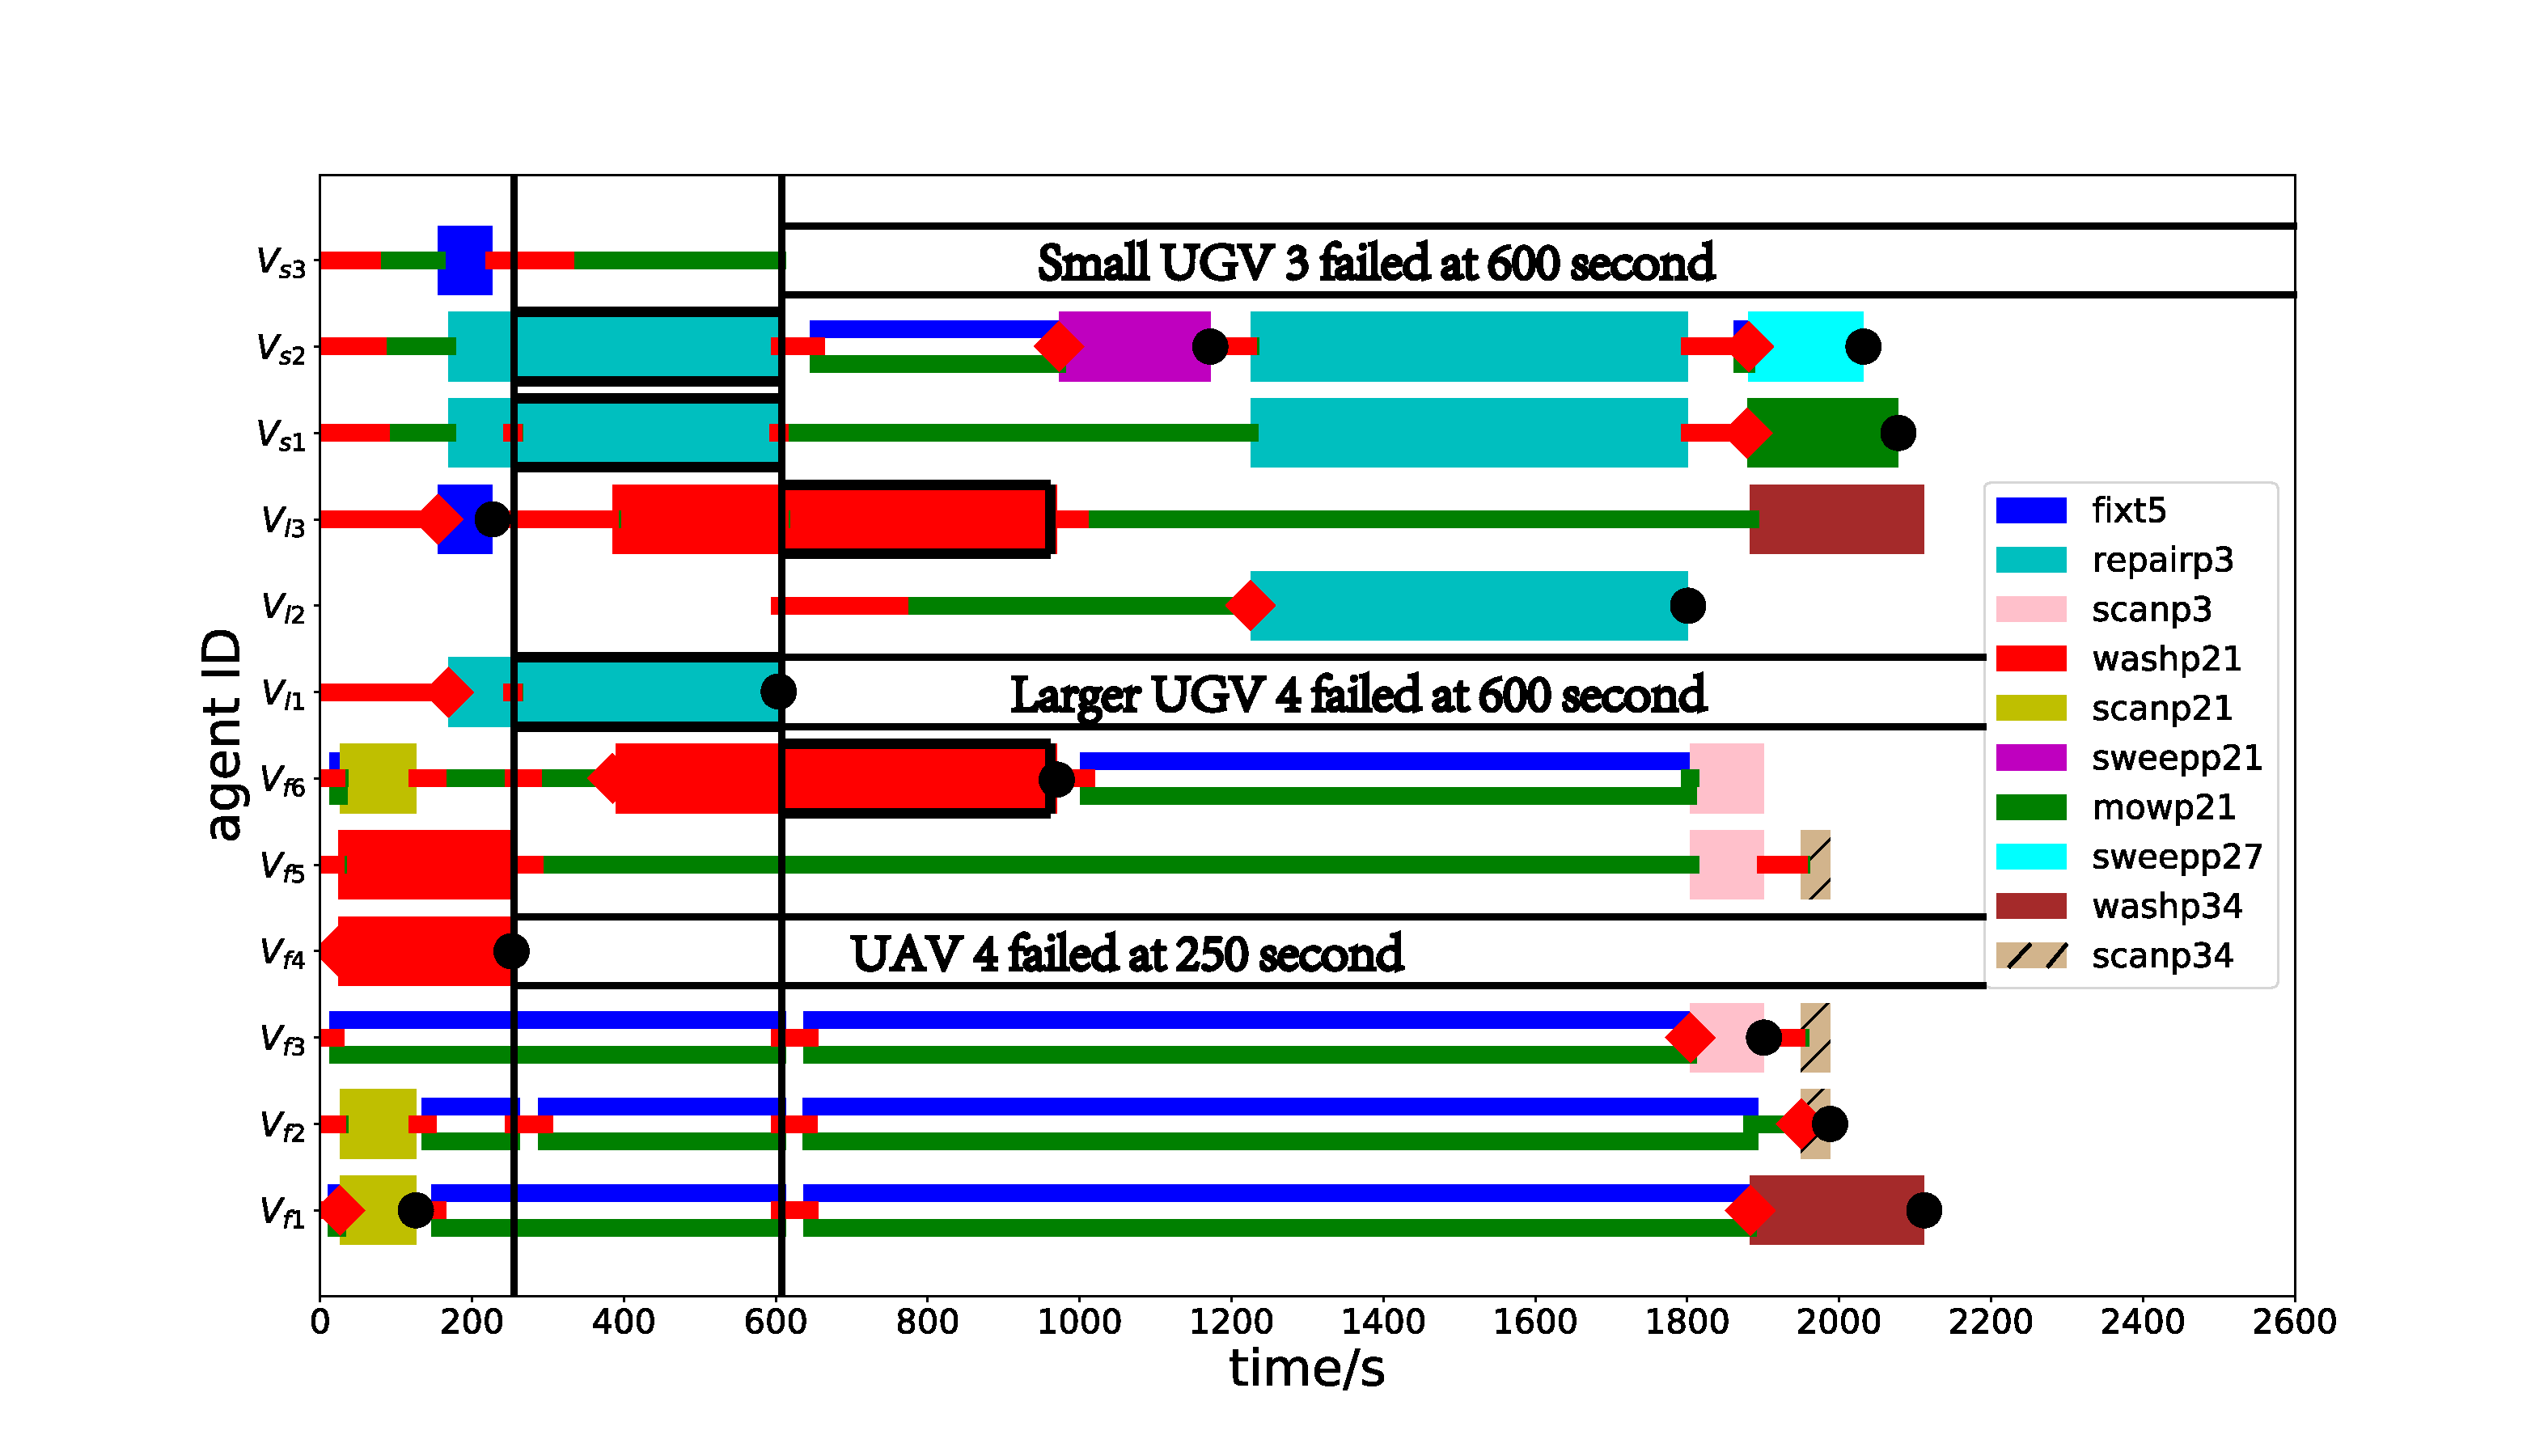
\includegraphics[scale=0.20]{figs/gantt_communicate1.pdf}
 	\caption{Exchange of ``start'' and ``stop'' messages.}
 	\label{fig:communicate}
\end{figure}


In addition, more explanations are added in Section 6.1:
\begin{itemize}
\item In the second paragraph, right column, Page 11,
it is clarified that the agent with the largest ID is chosen as the
temporary leader of the sub-group performing the subtask $\omega^k_n$,
and this leadership lasts until the end of this subtask.

\item In the third paragraph, right column, Page 11, it is emphasized that
  the communication of "\texttt{start}" and "\texttt{stop}" messages is performed only between leaders.

\item In the forth paragraph, right column, Page 11,
it is emphasized that
if~$\omega^k_n$ is a collaborative behavior, then
agent~$n$ sends another synchronization message to the leader agent
of this behavior to start executing this action.
The leader coordinates with all collaborators to start simultaneously
after relevant constraints within the R-posets are satisfied and
the synchronization messages of all collaborators are received.
\end{itemize}
$\hfill\blacksquare$

\hspace*{\fill} \

%===========================================================



%===========================================================


\textbf{C:}
\emph{In Eq. 12, how are the temporal order constraints on executing the
	tasks taken into consideration while estimating the concurrency using
	Eq. 12. Specifically, it is not quite clear how the highest concurrency
	is the criterion for choosing the next node to expand while taking into
	consideration that the temporal order constraint of the tasks are still
	satisfied.
}

\textbf{A:} Thanks for this insightful comment.
Equation (12) is used as a heuristic to choose the next node to expand,
which maximizes the concurrency of executing the remaining subtasks.
Actually, these temporal constraints are considered when computing $T_{\nu}$, i.e.,
\begin{equation*}\label{eq:node-makespan}
T_\nu = \max_{n\in\mathcal{N}} \{T_{\tau_n}\},\;
T^{\texttt{s}}_\nu = \sum_{\omega\in\Omega_\nu}\, D_{\omega}N_\omega,\;
\eta_\nu = \frac{T^{\texttt{s}}_\nu}{T_\nu};
\end{equation*}
where node~$\nu=(\tau_1,\cdots,\tau_N)$;~$T_{\tau_n}$ is the execution
time of all subtasks in~$\tau_n$ by agent~$n$; $T_\nu$ is the max makespan calculate by this equation,
and $T^{\texttt{s}}_\nu$ is the total execution time of all subtasks~$\omega$
given its duration~$D_\omega$ and the number of participants~$N_\omega$.
$T_{\nu}$ is calculated by considering the temporal constraints and the motion
constrains of the agents.

\begin{figure}[ht]
	\centering
	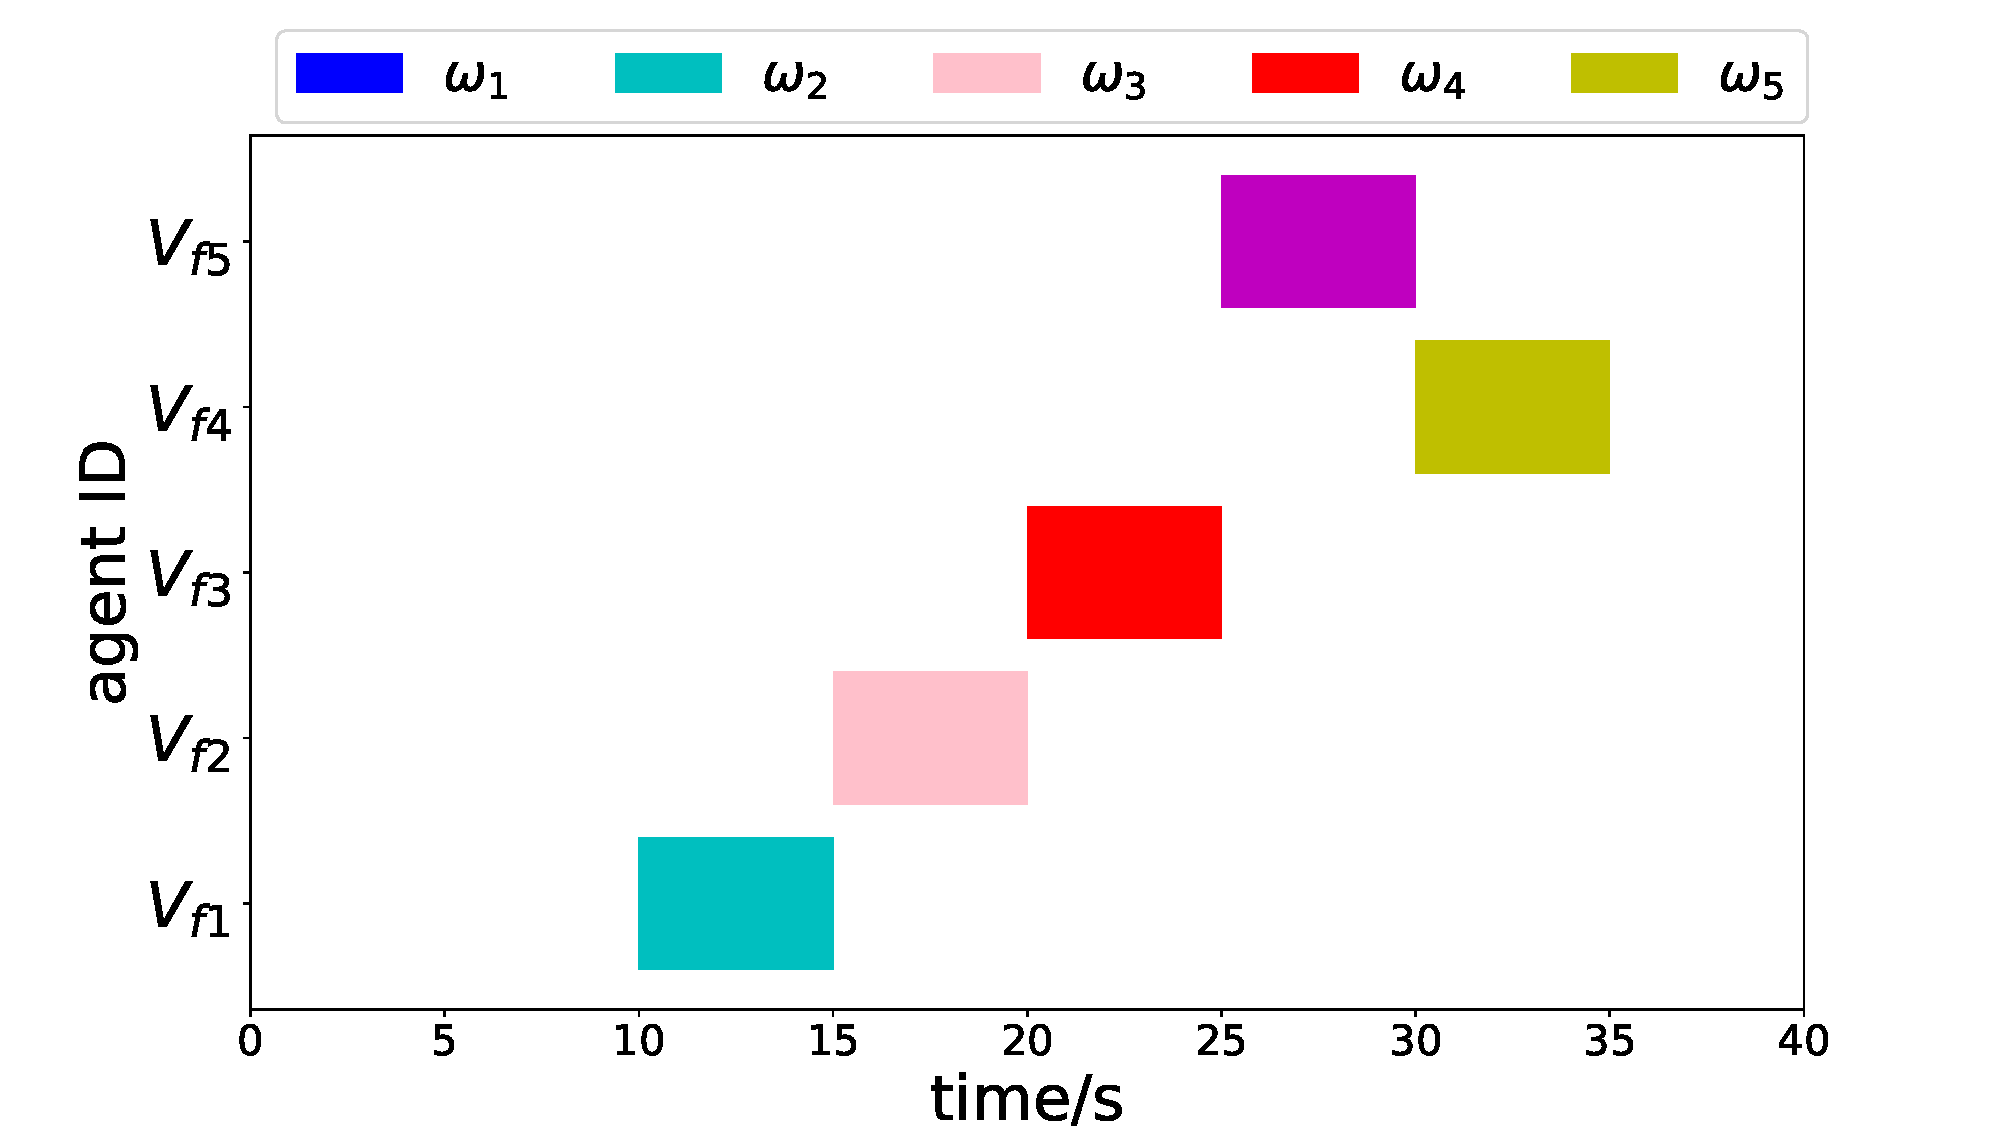
\includegraphics[scale=0.20]{figs/example_gantt.pdf}
	\caption{Gantt graph for task assignment.}
	\label{fig:gantt_example}
\end{figure}

For instance, consider the node $\nu=((\omega_1),(\omega_2),(\omega_3),(\omega_4),(\omega_5))$.
It takes each agent uniformly~$10s$ to reach the task region and the duration of each task is uniformly set to~$5s$.
In addition, the temporal constraints are given by~$\preceq=\{(\omega_1,\omega_2), (\omega_2,\omega_3), (\omega_3,\omega_4),(\omega_3,\omega_5)\}$,
and $\neq=\{(\omega_1,\omega_2),(\omega_2,\omega_3),
(\omega_3,\omega_4),(\omega_3,\omega_5),\\(\omega_4,\omega_5)\}$.
The optimal assignment is showed in Figure~\ref{fig:gantt_example} on the previous page.
Although each agent can arrive the task region at $10s$,
they need to wait until the temporal constraints are satisfied.
The subtask $\omega_4$ is executed by agent~$4$ after the subtask~$\omega_5$ is accomplished
due to the constraint that $(\omega_4,\omega_5)\not\in\preceq$ and $\omega_4\neq\omega_5$.
Then, the concurrency level is given by~$\eta_\nu=25/35=0.714$.
The higher $\eta_\nu$ is, the more efficient the node is.
We choose the node with higher $\eta_\nu$ instead of $T_\nu$, since
the comparison is made between different nodes.
The makespan $T_\nu$ only represents the efficiency
of nodes with the same set of assigned subtasks,
while the concurrency level $\eta_\nu$ can take into account different sets of assigned subtasks when comparing nodes.
Thus, the temporal constraints from R-poset are considered when computing~$\eta_{\nu}$ above.


The above explanations and more clarifications have been added into the manuscript; please refer to the colored sentences in last paragraph, Page 10, left column.
$\hfill\blacksquare$


\hspace*{\fill} \

%===========================================================

\textbf{C:}
\emph{
	The authors are suggested to expand the descriptions on the future
	work. "Future work includes the distributed variant." is a bit terse.
}

\textbf{A:} As suggested, the descriptions on the future
work have been expanded.  Specifically, future work includes the distributed methods for computing
	the products between local and global R-posets.
	This can potentially alleviate the complexity bottleneck
	when translating a long LTL formula into its associated NBA.
These details have been added into the Conclusion section on Page 16.
$\hfill\blacksquare$




\newpage
\section*{To Reviewer 6}

\textbf{C:}
\emph{
The authors present a novel anytime planning algorithm for multi-agent
task assignment and planning. On top of that, they provide an online
adaption algorithm to replan and reschedule in case of execution length
fluctuation or complete task failure. The authors analyze their
algorithm with regard to soundness, completeness and optimality. The
authors provide numerical simulations and simulated usecase scenarios,
comparing to implementations of related works.}

\emph{
The authors introduce the topic well and list sufficient relevant
related works and how they are comparable. Especially Table 1 is very
useful. To the best of my knowledge, no obviously relevant work is
missing.}

\emph{
The technical contribution of this work explained rigorously and all
parts of the algorithm are explained in detail. A few sections were
hard to follow or unclear, but none of these are major issues (please
see the details). One of the biggest strengths of this work is the
comparison to related methods. The authors took time and effort to
implement a total of four different baseline algorithms in addition to
their own.}

\emph{
Throughout the non-technical sections, the writing contains many
grammatical errors and odd formulations. For example, I generally
recommend using active formulation to provide better readability. ("We
show XYZ" instead of "XYZ is shown"). Details can be found in the
attachment, but I advise the authors to carefully revise the writing of
the manuscript section by section, as I was not able to list all
occurences. }

\emph{
I hope the attached details.pdf can be helpful to the authors.
}



\textbf{A:}
The authors thank the reviewer for the constructive comments and insightful suggestions.
They helped us greatly improve the submission and further strengthen its contributions.
In addition,
we have changed numerous passive voices into active in the Introduction, e.g.,
``The overall algorithm is proven'' is changed to
``We prove'';
``Besides, an online synchronization protocol is proposed''
is changed to
``Besides, we propose an online synchronization protocol'';
and ``an adaptation algorithm is proposed'' is changed to
``we propose an adaptation algorithm''.
Furthermore,
the mentioned grammatical errors have been corrected.

Below we summarize our replies to these comments, accompanied by the list of changes in the revision.
All these changes have been highlighted in blue in the revised paper.
$\hfill\blacksquare$

\hspace*{\fill} \

%===========================================================

\textbf{C:}
\emph{ "Multi-agent systems can be EXTREMELY efficient ...", "Both algorithms are validated
	RIGOROUSLY [...], against STRONG baselines": The abstract contains multiple instances of
	emotional, strong adjectives that are not based on factual evidence, most likely to
	strengthen the selling points of the work. I advise revising this type of language to remain
	rational.
}

\textbf{A:} Thanks for your suggestions.
We have tuned down the subjective descriptions and instead emphasized more the factual evidences.
More specifically,
``extremely'' has been removed and the last sentence in the {Abstract} has been modified to
``Both algorithms are validated over systems of more than $10$ agents via numerical simulations and hardware experiments, against several baselines.''
$\hfill\blacksquare$



\hspace*{\fill} \

%===========================================================

\textbf{C:}
\emph{"Analyses of its soundness, completeness and optimality as the minimal completion time are
	provided.": I recommend reformulating this sentence, e.g. into "We analyze soundness,
	completeness and optimality with regard to minimal completion time."
}

\emph{ "It is also shown ..." $\rightarrow$ "We show ..."
}

\emph{ "... an adaption algorithm is proposed" $\rightarrow$ "We propose ..."
}

\textbf{A:} Thanks for your suggestions.
We have changed numerous statements into active voice whenever appropriate.
For instances,
besides the ones suggested above, we have changed other sentences into active voice as follows:
\begin{itemize}
\item On Page 2,  left column, the description
is changed to ``We give the team-wise task as LTL formulas over the desired
actions to perform at the desired regions of interest in the environment''.

\item On Page 2,  left column, we have changed the contributions to
``We prove the completeness and soundness of the overall algorithm for the considered objective,
and we also show empirically that algorithm can quickly reach a feasible and near-optimal solution".

\item On Page 2,  left column,  the description is changed to ``Besides,
we propose an online synchronization protocol to handle fluctuations in the execution time,
while ensuring that the partial ordering constraints are still respected".


\item On Page 2,  left column,  the statement is changed to
``we propose an adaptation algorithm to synchronize execution status and re-assign unfinished subtasks dynamically to maintain correctness and optimality''.
\end{itemize}

$\hfill\blacksquare$



\hspace*{\fill} \

%===========================================================


%===========================================================

\textbf{C:}
\emph{ "It is particularly so when certain metric should be minimized, such as the completion time or
	the summed cost of all robots.": Metrics should be plural}

\textbf{A:} Thanks for pointing this out. We have fixed the grammatical error.
$\hfill\blacksquare$

\hspace*{\fill} \

%===========================================================

\textbf{C:}
\emph{ "It is particularly so when..." $\rightarrow$ "This is particularly the case when..."
}


\textbf{A:} Thanks for pointing this out. We have fixed the typo.
$\hfill\blacksquare$

\hspace*{\fill} \

%===========================================================

\textbf{C:}
\emph{"Each of these two sub-routines is anytime itself"
	I understand anytime comes from anytime-algorithms, but I would recommend against using
	the word anytime like this. Maybe "Both subroutines are anytime-algorithms"?
}

\textbf{A:} Thanks for the suggestion. We have modified the sentence accordingly.
$\hfill\blacksquare$

\hspace*{\fill} \

%===========================================================

\textbf{C:}
\emph{The section name of ``preliminarie'' should be plural.
}


\textbf{A:} Thanks for the detailed comment. We have fixed the typo.
$\hfill\blacksquare$

\hspace*{\fill} \

%===========================================================

\textbf{C:}
\emph{ When introducing co-safe LTL, please provide a reference containing a formal definition
}

\textbf{A:} Thanks for your suggestion.
We have added the new reference (Belta et al., 2017).
In particular, Definition 2.3 on Page 30 of this reference is referred to
as the exact definition of syntactically co-safe LTL. This reference is cited in the second paragraph, right column, Page 3.
$\hfill\blacksquare$

\hspace*{\fill} \

%===========================================================

\textbf{C:}
\emph{ Positive normal form is not explained and might not be clear to every reader.
}

\textbf{A:} Thanks for this comment.
We have provided more details regarding the definition of positive normal form.
Namely, the negation operator $\neg$ can appear only in
front of labels, while not $\Diamond, \bigcirc, \textsf{U}$.
Detailed changes can be found in the second paragraph, right column, Page 3, as follows:
They only contain the temporal operators $\bigcirc$, $\textsf{U}$ and $\Diamond$
and are written in positive normal form where the negation
	operator $\neg$ is not allowed before the temporal
	operators including~$\bigcirc, \textsf{U}, \Diamond$.
$\hfill\blacksquare$

\hspace*{\fill} \

%===========================================================

\textbf{C:}
\emph{In an NBA, there exists not "the" resulting run, but a set of possible resulting runs.
}

\textbf{A:} Thanks for pointing this out.
We have modified the description as follows in the fifth paragraph, right column, Page 3, as follows:
``Given an infinite word $w=\sigma_1\sigma_2\cdots$, we can get a set of
 resulting \emph{run} within $\mathcal{B}$.
Each of them is an infinite sequence $\rho=q_0q_1q_2\cdots$.''
$\hfill\blacksquare$

\hspace*{\fill} \

%===========================================================

\textbf{C:}
\emph{ When informally introducing the concept that every omega-regular property can be divided
	into a prefix and repeated suffix, please provide a reference to formal proof. Baier \& Katoen
	2008 have this proof and is already cited further above.}

\textbf{A:} Thanks for this comment. As suggested, we have added the reference (Baier \& Katoen
2008) in the fifth paragraph, right column, Page 3.
$\hfill\blacksquare$

\hspace*{\fill} \

%===========================================================

\textbf{C:}
\emph{While every omega-regular property can be expressed through a prefix-suffix-pair, not every
	accepting run has to be in such form, especially when the NBA is not finite.
}

\textbf{A:} Thank you for your comment. We have rephrased this part and point out
the differences between LTL and sc-LTL in the last paragraph in Section 3.2 on Page 3.
Namely, the set of all words that correspond to the \emph{accepting} runs is called
the \emph{language} generated by the NBA. The language can be expressed
in the prefix-suffix structure~(Baier \& Katoen, 2008), while the prefix part
can result in a run from an initial state to an accepting state, and the suffix
part can result in a cyclic run that contains the same accepting state.
Moreover, the
satisfaction of a sc-LTL formula can be achieved in a finite time, i.e.,
each word satisfying a sc-LTL formula consists of a satisfying prefix that
can be followed by an arbitrary suffix.
$\hfill\blacksquare$

\hspace*{\fill} \

%===========================================================

\textbf{C:}
\emph{"...if the prefix is repeated once": confusing formulation. The prefix does not need to be
	repeated
}

\textbf{A:} Thanks for pointing this out. You are right that the prefix does not repeat.
To avoid confusion, we have deleted the relevant expression from the point view of a run.
Instead, we re-state it from the perspective of a word. Please refer to the colored sentences in the last paragraph in Section 3.2, Page 3.
$\hfill\blacksquare$

\hspace*{\fill} \

%===========================================================

\textbf{C:}
\emph{the team-wide task specification is defined in sc-LTL, but the preliminaries call it co-safe LTL.
}

\textbf{A:} Thanks for the detailed comment. We have fixed the typo and unified the term as ``sc-LTL''.
Detailed changes can be found in the second paragraph, right column, Page 3
and in the last paragraph, left column, Page 4.
$\hfill\blacksquare$

\hspace*{\fill} \

%===========================================================
\textbf{C:}
\emph{ "with more than $1.29 x 10^7$ word": words should be plural.}

\textbf{A:} Thanks for pointing this out. We have fixed this error.
$\hfill\blacksquare$

\hspace*{\fill} \

%===========================================================

\textbf{C:}
\emph{ "Without losing any information": pruning decomposable edges and thus removing accepting
	words does change the accepted language and thus loses information. I understand why
	decomposable transitions can be removed in this scenario, but calling it "not losing
	information" is not correct.
}

\textbf{A:} Thanks for this insightful comment.
Indeed, pruning by removing certain edges does actually reduce the set of accepting words,
i.e., certain information is lost from this perspective.
However, as you mentioned, the property mentioned in Lemma 1 has proven that
if there exists a word $w$ that is accepted by $\mathcal{B}$,
an equivalent word $w'$ can be found that is accepted
by the pruned NBA $\mathcal{B}^-$.
For the sake of accuracy, we have
removed this statement.
$\hfill\blacksquare$

\hspace*{\fill} \

%===========================================================
\textbf{C:}
\emph{What if states in the NBA does not have a self-loop? Can a subtask still be defined? For
	example the formula $a \& X b$ should result in an automaton with multiple states without
	self-loop. I recommend looking into stutter-free properties (e.g. by omitting the next
	operator), as they should result in automata where every state has a self-loop. }

\textbf{A:} Thanks for this insightful comment. The existence of self loops in the definition of subtasks
is actually not strictly required.
Namely, when a loop does not exist over one vertex, it means that no label constraints are imposed before the execution
of the current subtask. But it requires that this subtask should start being executed after the start of the prior subtask and before it is finished. In general,
we define $\sigma^s_\ell$ as $\{Null\}$ to represent that there is no self loop over one vertex.
In your example $\varphi=a\bigcirc b$,
the associated NBA is shown with three states the Figure~\ref{fig:anextb} on the next page. As both states $init$ and $1$ have no
self loops, their labels are set to~$\sigma^s_1=\sigma^s_2=\{Null\}$,
meaning that self loops do not exist.
Then, we can create two subtasks as $\Omega_\varphi=\{\omega_1=(1,\{a\},\{Null\}),  \omega_2=(2,\{b\},\{Null\})\}$.
We have added this explanation in the last paragraph, left column, Page 6.
\begin{figure}[ht]
	\centering
	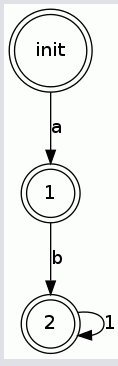
\includegraphics[scale=0.35]{figs/aob.png}
	\caption{A pruned B\"{u}chi automaton.}
	\label{fig:anextb}
\end{figure}
$\hfill\blacksquare$


\hspace*{\fill} \

%===========================================================

\textbf{C:}
\emph{"Thus, the probability of two actions are fulfilled at the exact time instant is of measure
	zero.": This argument stemming from continuous time does not hold when considering
	discrete instances in time. Is this really correct here?
}

\textbf{A:} Thanks for your insightful comment. Our description
here is indeed inaccurate.
The purpose of this statement is to motivate that most existing work only takes into account tasks that can be accomplished instantaneously,
i.e., instead of a task with duration.
Thus, only the ``less equal'' relation is considered in related work,
without the ``opposed''  relation.
To avoid confusion, we have instead directly pointed out that related works assume an essential sequence of subtasks,
while ignoring the conflicting labels.
These explanations have been added into the manuscript; please refer to the colored sentences in Remark 3  on Page 6.
$\hfill\blacksquare$

\hspace*{\fill} \

%===========================================================


\begin{figure}[ht]
	\centering
	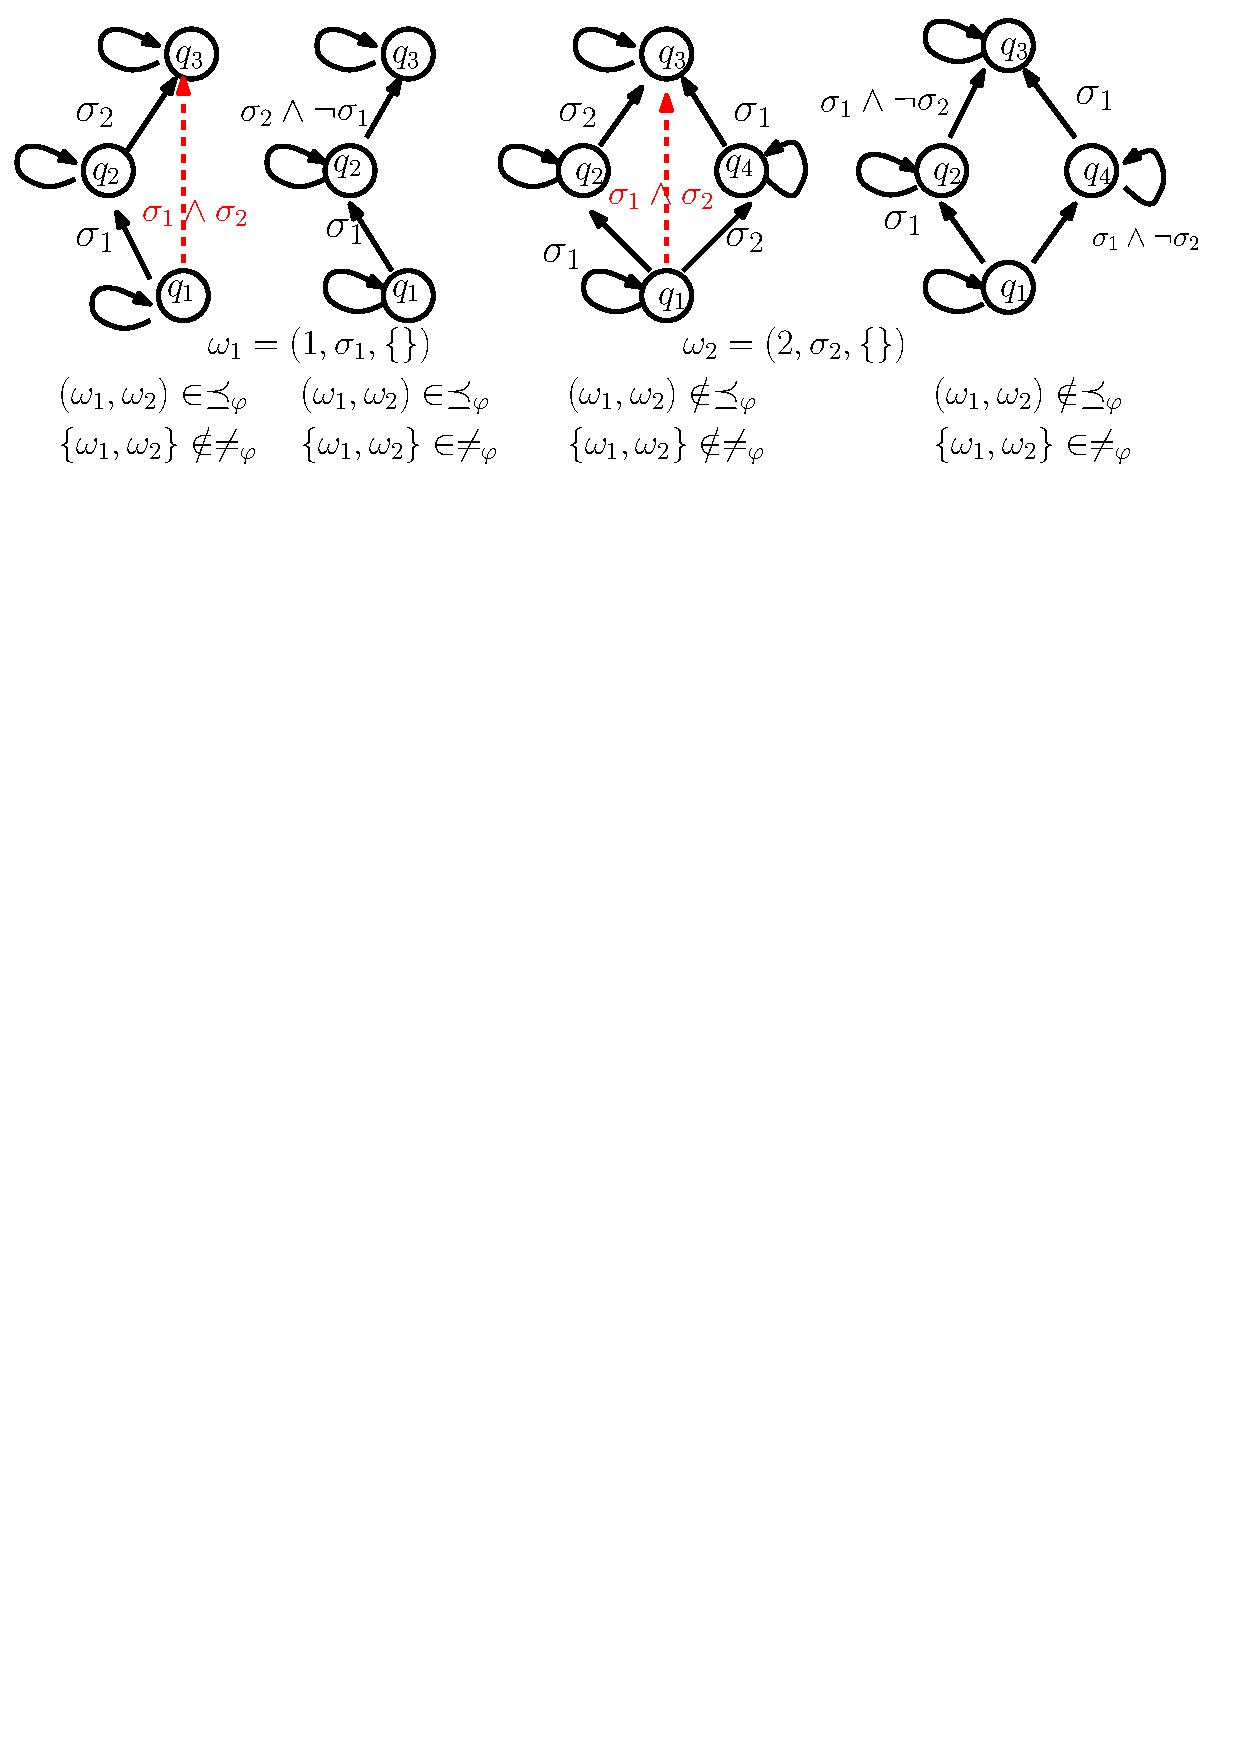
\includegraphics[scale=0.5]{figs/explain_about_remark4.pdf}
	\caption{$\preceq_\varphi$, $\neq_\varphi$ relations in a pruned NBA.}
	\label{fig:example_remark_4}
\end{figure}


\textbf{C:}
\emph{ I was not able to follow the reasoning between definition 5 and remark 4.
}

\textbf{A:} Thank you for your review.
The purpose of Remark 4 is to motivate why these two specific relations $\preceq_\varphi, \preceq_\varphi$ are chosen
when defining the R-poset in Definition 5.
Namely, these two relations $\preceq_\varphi$ and $\neq_\varphi$
are chosen in the definition of R-posets due to the following observations:
Firstly, these two relations can accurately describe the relationship
between non-instantaneous tasks in a continuous-time system.
There are four possible temporal orders between two subtasks $\omega_1,\omega_2$:
(i) $\omega_2$ should be executed after $\omega_1$ has begun, i.e., ($\omega_1,\omega_2)\in\preceq_{\varphi},\{\omega_1,\omega_2\}\notin\neq_\varphi$;
(ii) $\omega_2$ should be executed after $\omega_1$ has ended, i.e.,
$(\omega_1,\omega_2)\in\preceq_{\varphi}, \{\omega_1,\omega_2\}\in\neq_\varphi$;
(iii) $\omega_1$ and $\omega_2$ can not be executed at the same time,
i.e., $(\omega_1,\omega_2)\notin\preceq_\varphi,\{\omega_1,\omega_2\}\in\neq_\varphi$;
(iv) $\omega_1$ is parallel to $\omega_2$, i.e., $(\omega_1,\omega_2)\notin\preceq_\varphi,
\{\omega_1,\omega_2\}\notin\neq_\varphi$.
Secondly, these two relations can preserve the key information in the
pruned NBA.
As illustrated in Figure~\ref{fig:example_remark_4} on the previous page, %这个fig:example_remark_4 是这里的图,不是引用论文的图
$\preceq_\varphi,\neq_\varphi$ can not only
describe whether the subtasks can switch their orders,
but also indicate whether they can be executed simultaneously.
Last but not least, it is proved in Lemma 2 that any word satisfying
the constraints $\preceq_\varphi, \neq_\varphi$ of R-poset can be
generated by a switching sequence from the original word.
Thus, a word is accepting only if it satisfies these relations of an accepting R-poset.
These clarifications have been added into Remark 4 on Page 7.
$\hfill\blacksquare$

\hspace*{\fill} \


\textbf{C:}
\emph{ "..., we assign only the next task satisfies the partial order.": This sentence is clearly missing a
	word
}

\textbf{A:} Thanks for this detailed comment. We have fixed the grammatical mistake.
$\hfill\blacksquare$

\hspace*{\fill} \

\textbf{C:}
\emph{Variable time is never updated
}

\textbf{A:} Thanks for pointing this out. The elapsed time is now updated within the ``while'' loop; see Line $30$ of Algorithm 1 on Page 8.
$\hfill\blacksquare$

\hspace*{\fill} \

 \textbf{C:}
\emph{Can you guarantee one iteration of the outer while-loop is completed fast enough? Is
	constructing the initial poset always quick enough? }

\textbf{A:} Thanks for your insightful comment.
In general, the complexity of one iteration within the main while loop
is determined by the size of R-poset.
Firstly, a DFS method is applied to find a
new accepting run $\rho$ when computing one R-poset.
This means that one R-poset can be derived
once a new accepting run with the word
$w\notin\mathcal{L}_\varphi$ is found, instead of the complete set of words.
Secondly, the relations $\preceq_\varphi$, $\neq_\varphi$ and $\sigma^s_\ell$ are calculated by repetitively checking
whether the switched word $w'$ can be accepted.
The total number of iterations depends on the size of the language associated with the R-poset.
For instance,
if the set of language is small with $|L(P)|=1$, the calculation is done with one iteration.
On the other hand, if there are no partial ordering constraints that $|\preceq_\varphi|=0$,
the set of language is large as $|L(P)|=|\Omega_\varphi|!$.
In our numerical tests,
the initial R-poset is found in seconds for a language of around
$600$ words.

Moreover, the speed of constructing the initial poset is also determined by the size of the R-poset constructed in the first found word.
But in the worst case that the pruned NBA has only one R-poset, its complexity will not exceed the complexity of finding
all the accepting words by DFS, because in the worst case, we will
search for all feasible words, and all of them are accepting.
Thus, we have revised the relevant statements to make them more accurate;
please refer to the colored sentence in the third paragraph, Page 7, right column.

Lastly, to ensure that the algorithm is a strictly anytime algorithm during the computation of the R-poset,
we have added an additional condition inside the main loop
such that once the computation time is up, the algorithm returns
the sets $\mathcal{P}_{\varphi},\mathcal{L}_\varphi$; please refer to Line 20 of Algorithm 1.
$\hfill\blacksquare$

\hspace*{\fill} \

\textbf{C:}
\emph{The self-loop is computed by checking all feasible words. Is this computationally efficient?
	The number of feasible words should grow quite quickly in scenarios with little constraints.}

\textbf{A:} Thanks for this insightful comment.
 The self loop associated with each node can be
computed in an efficient way.
To begin with, we do not check all feasible words,
instead only the feasible ones in $L(P)$.
Second, the set $L(P)$ is already derived
when computing $\preceq$, thus no extra time is needed.
Third, the step $\sigma^p_{\ell_i}=\sigma^p_{\ell_i}\cap\delta^{-1}(\rho'[i-1],\, \rho'[i-1])$
in Line 28 of Algorithm 1 is only performed when different self loops exist.
Generally speaking,
the derived $\delta^{-1}(\rho'[i-1],\rho'[i-1])$ is stored during
the computation of $\sigma^s_{\ell_i}$.
Thus, if a new self loop $\delta^{-1}(\rho[i-1], \rho[i-1])$ has already been calculated,
this step in Line 28 will be skipped directly.
In other words, although the complete set of language $P$ can be
large in scenarios with few constraints,
the number of times when self loops are derived is rather limited.
In our numerical tests,
the self loop can be found in seconds for a language of around
$5000$ words.
$\hfill\blacksquare$

\hspace*{\fill} \


\textbf{C:}
\emph{ possible typo with two subsequent $\subset$}

\textbf{A:} Thanks for pointing out this typo, which has been corrected in this revision.
$\hfill\blacksquare$

\hspace*{\fill} \

\textbf{C:}
\emph{ Discussion for future work is a single sentence with 6 words. This should be either expanded
	or entirely left out, as it currently does not contribute much to the paper}

\textbf{A:} Thanks for your suggestion.
The descriptions on the future
work have been expanded.  Specifically, future work includes the distributed methods for computing
the products between local and global R-posets.
This can potentially alleviate the complexity bottleneck
when translating a long LTL formula into its associated NBA.
These details have been added into the Conclusion section on Page 16.
$\hfill\blacksquare$

\end{document}
